
\newpage
\subsection{Scalar AES Acceleration}
\label{sec:scalar:aes}

This section details proposals for acceleration of
the AES block cipher \cite{nist:fips:197} within a scalar RISC-V core,
obeying the two-read-one-write constraint on general purpose register
file accesses.
Performance and RTL benchmarks for these
instruction proposals are found in Section
\ref{sec:benchmark:aes}.

\subsubsection{RV32 Instructions}
\label{sec:scalar:aes:rv32}

\begin{cryptoisa}
saes32.encs      rd, rs1, rs2, bs // Encrypt: SubBytes
saes32.encsm     rd, rs1, rs2, bs // Encrypt: SubBytes & MixColumns
saes32.decs      rd, rs1, rs2, bs // Decrypt: SubBytes
saes32.decsm     rd, rs1, rs2, bs // Decrypt: SubBytes & MixColumns
\end{cryptoisa}

These instructions are a very lightweight proposal, derived from
\cite{MJS:LWAES:20}.
They are designed to enable a partial T-Table based implementation
of AES in hardware, where the SubBytes, ShiftRows and MixColumns
transformations are all rolled into a single instruction, with the
per-byte results then accumulated.
The {\tt bs} immediate operand is a 2-bit {\em Byte Select}, and indicates
which byte of the input word is operated on.
Pseudo-code for each instruction is found in figure
\ref{fig:pseudo:aes:rv32}.

\begin{figure}[h]
\begin{lstlisting}[language=pseudo]
saes32.encs(rs1, rs2, bs):                 // SubBytes Only
    t0.8  = rs2.8[bs]
    x.8   = AESSBox(t0)
    u.32  = {0, 0, 0, x}
    rd.32 = ROTL32(u, 8*bs) ^ rs1.32

saes32.encsm(rs1, rs2, bs):                // SubBytes & MixColumns
    t0.8  = rs2.8[bs]
    x.8   = AESSBox(t0)
    u.32  = {GFMUL(x,3) , x, x, GFMUL(x,2)}
    rd.32 = ROTL32(u, 8*bs) ^ rs1.32

saes32.decs(rs1, rs2, bs):                 // InvSubBytes Only
    t0.8  = rs2.8[bs]
    x.8   = InvAESSBox(t0)
    u.32  = {0, 0, 0, x}
    rd.32 = ROTL32(u, 8*bs) ^ rs1.32

saes32.decsm(rs1, rs2, bs):                // InvSubBytes & InvMixColumns
    t0.8  = rs2.8[bs]
    x.8   = InvAESSBox(t0)
    u.32  = {GFMUL(x,11),GFMUL(x,13),GFMUL(9),GFMUL(14)}
    rd.32 = ROTL32(u, 8*bs) ^ rs1.32
\end{lstlisting}
\caption{Pseudocode for the lightweight AES instructions targeting the
RV32 base architecture.}
\label{fig:pseudo:aes:rv32}
\end{figure}

\note{
The SM4 (see Section \ref{sec:scalar:sm4}) and RV32 AES 
instructions are designed to share much of their datapath, and
can be implemented with much logic shared  between their SBoxes
in particular.
}


% ------------------------------------------------------------

\newpage
\subsubsection{RV64 Instructions}
\label{sec:scalar:aes:rv64}

\begin{cryptoisa}
saes64.ks1      rd, rs1, rcon  // KeySchedule: SubBytes, Rotate, Round Const
saes64.ks2      rd, rs1, rs2   // KeySchedule: XOR sumation.

saes64.encsm.lo rd, rs1, rs2   // Encrypt ShiftRows, SubBytes, MixColumns
saes64.encsm.hi rd, rs1, rs2   //
saes64.encs.lo  rd, rs1, rs2   // Encrypt ShiftRows, SubBytes
saes64.encs.hi  rd, rs1, rs2   //

saes64.imix     rd, rs1        // InvMixColumns for Decrypt KeySchedule
saes64.decsm.lo rd, rs1, rs2   // Decrypt ShiftRows, SubBytes, MixColumns
saes64.decsm.hi rd, rs1, rs2   //
saes64.decs.lo  rd, rs1, rs2   // Decrypt ShiftRows, SubBytes
saes64.decs.hi  rd, rs1, rs2   //
\end{cryptoisa}

These instructions are for RV64 only.
They implement the SubBytes, ShiftRows and MixColumns transformations of AES
over two instructions.
Each instruction takes two 64-bit registers as input, which represents
the entire 128 bit state of the AES cipher.
The instructions use the equivalent inverse cipher construction
\cite[Page 23, Section 5.3.5]{nist:fips:197}.
Hence there are additional instruction specifically for performing the
inverse MixColumns transformation as part of the modified key schedule.
The byte mapping of input register values to AES state and output register
values is shown in \figref{aes:rv64:mapping}.
Pseudocode for the instructions is illustrated in
\figref{pesudo:aes:rv64}.

These instructions are designed to be implemented using macro-op fusion or
operand memoisation.
This is similar to the recommended \mnemonic{mulh}, \mnemonic{mul}
sequence in the M extension to compute a full $32*32->64$ bit
multiplication result \cite[Section 7.1]{riscv:spec:user}.

\begin{itemize}
\item
The {\tt *.lo} variants compute the first 8 bytes of the next round
state, while the {\tt *.hi} variants compute the last 8 bytes of the
next round state.
By performing the (Inverse) ShiftRows transformation before the
(Inverse) SubBytes transformation, no SubBytes computations need to be
thrown away.
In this way, the {\tt *.lo/*.hi} encoding bit acts as an input selector.
See the pseudocode in \figref{pesudo:aes:rv64} to see how this works.
\item
The \mnemonic{saes64.encsm.*}/\mnemonic{saes64.decsm.*} instructions perform the
(Inverse) SubBytes, ShiftRows and MixColumns Transformations.
\item
The \mnemonic{saes64.encs.*}/\mnemonic{saes64.decs.*} instructions perform the
(Inverse) SubBytes and ShiftRows Transformations.
They are used for the last round of AES only.
\item
The \mnemonic{saes64.ks1}/\mnemonic{saes64.ks2} instructions are used in the
KeySchedule.
\mnemonic{saes64.ks1} implements the rotation, SubBytes and Round Constant
addition steps.
\mnemonic{saes64.ks2} implements the remaining {\tt xor} operations.
\item
The \mnemonic{saes64.imix} instruction applies only the inverse MixColumns
transformation to two columns of the state array, packed into a single
64-bit register.
It is used to create the inverse cipher key schedule, according to
the equivalent inverse cipher construction in
\cite[Page 23, Section 5.3.5]{nist:fips:197}.
\end{itemize}

This proposal requires $6$ instructions per AES round:
$2$ \mnemonic{ld} instructions to load the round key,
$2$ \mnemonic{xor} to add the round key to the current state
and
$2$ of the relevent AES encrypt/decrypt instructions to perform the
    SubBytes, ShiftRows and MixColumns round functions.
This adds up to approximately $80$ instructions per AES-128 block
encryption, including pre/post-amble instructions.

\begin{figure}[h]
\centering
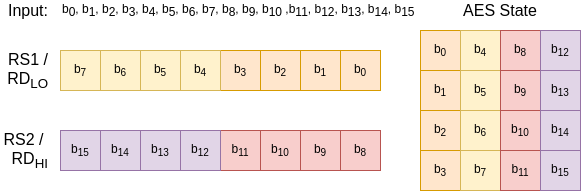
\includegraphics[width=0.8\textwidth]{diagrams/aes-rv64-state.png}
\caption{
Mapping of AES state between input and output registers for
the \mnemonic{saes64.enc.*} and \mnemonic{saes64.dec.*} instructions.
$RD_{LO}$ and $RD_{HI}$ are the output of \mnemonic{saes64.*.lo}
and \mnemonic{saes64.*.hi} instructions respectivley.
}
\label{fig:aes:rv64:mapping}
\end{figure}

\begin{figure}[h!]
\begin{lstlisting}[language=pseudo]
saes64.ks1(rs1,enc_rcon):      // KeySchedule: SubBytes, Rotate, Round Const
    temp.32   = rs1.32[1]
    rcon      = 0x0
    if(enc_rcon != 0xA):
        temp.32 = ROTR32(temp.32, 8)
        rcon    = AESRoundConstants.8[enc_rcon]
    temp.8[i] = AESSBox(temp.8[i])  for i=0..3
    temp.8[0] = temp.8[i  ] ^ rcon
    rd.64     = {temp.32, temp.32}

saes64.ks2(rs1,rs2):           // KeySchedule: XOR
    rd.32[0]  = rs1.32[1] ^ rs2.32[0]
    rd.32[1]  = rs1.32[1] ^ rs2.32[0] ^ rs2.32[1]

saes64.enc(rs1, rs2, mix, hi): // SubBytes, ShiftRows, MixColumns
    t1.128    = AESShiftRows(rs2 || rs1)
    t2.64     = t1.64[1] if hi else t1.64[0]
    t3.8[i]   = AESSBox(t2.8[i]) for i=0..7
    rd.32[0]  = AESMixColumn(t3.32[0]) if mix else t3.32[0]
    rd.32[1]  = AESMixColumn(t3.32[1]) if mix else t3.32[1]

saes64.dec(rs1, rs2, mix, hi): // InvSubBytes, InvShiftRows, InvMixColumns
    t1.128    = InvAESShiftRows(rs2 || rs1)
    t2.64     = t1.64[1] if hi else t1.64[0]
    t3.8[i]   = InvAESSBox(t2.8[i]) for i=0..7
    rd.32[0]  = InvAESMixColumn(t3.32[0]) if mix else t3.32[0]
    rd.32[1]  = InvAESMixColumn(t3.32[1]) if mix else t3.32[1]

saes64.imix(rs1):              // Inverse MixColumns
    rd.32[0]  = InvAESMixColumn(rs1.32[0])
    rd.32[1]  = InvAESMixColumn(rs1.32[1])
\end{lstlisting}
\caption{
RV64 AES instruction pseudocode.
Note how the $128$-bit {\tt [Inv]AESShiftRows} result in {\tt t1} has
either the high or low $64$ bits selected for further processing.
}
\label{fig:pesudo:aes:rv64}
\end{figure}

